%% Figure 2: how the same body of methods is organised in each tool.
%%
%% The point of the figure is the direction of composition, not a claim that
%% one organisation is better. On the left each analysis is a named command
%% that owns its own input handling, search and scoring. On the right the same
%% analyses are cells of a product of three axes, over shared machinery.

\documentclass[border=6pt]{standalone}
\usepackage{tikz}
\usepackage{amssymb}
\usetikzlibrary{arrows.meta,positioning,fit,backgrounds}
\providecommand{\code}[1]{\texttt{#1}}
\begin{document}
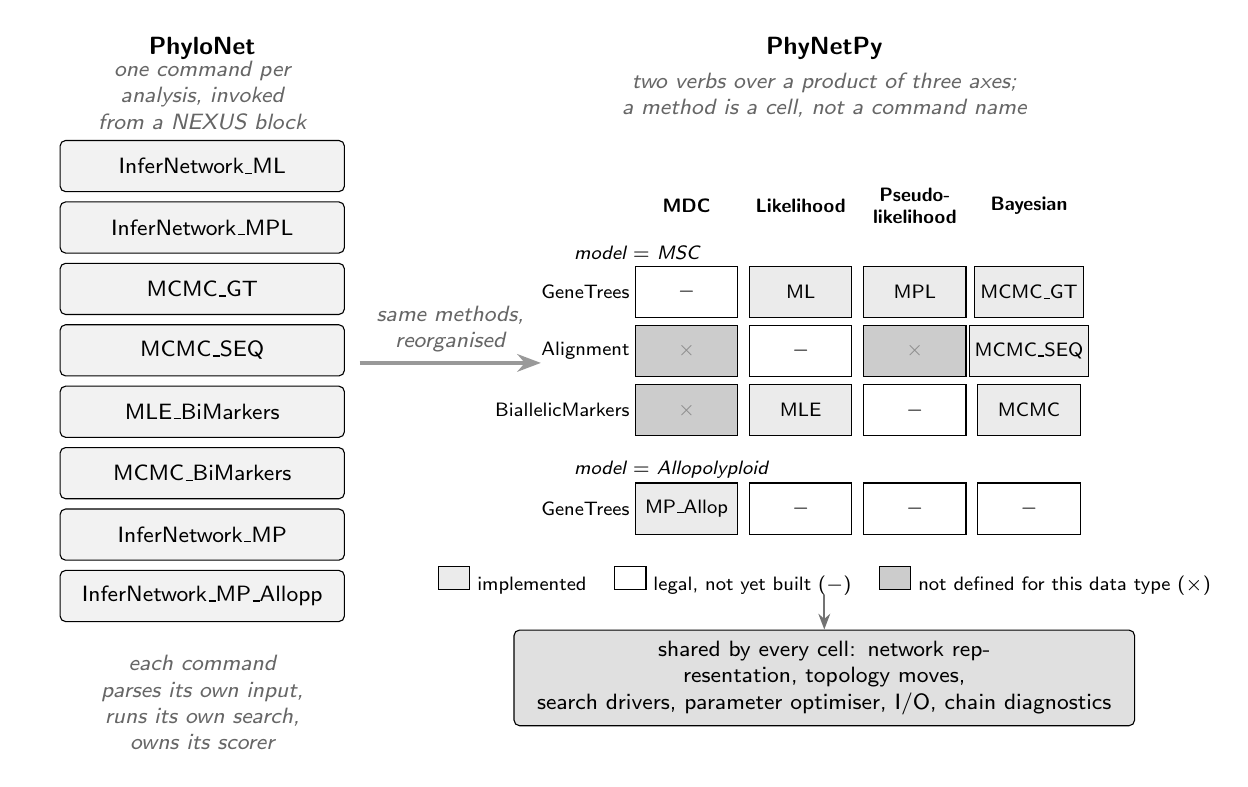
\begin{tikzpicture}[
  font=\sffamily\small,
  cmd/.style={
    draw, rounded corners=2pt, align=center, fill=black!5,
    text width=34mm, minimum height=6.5mm, inner sep=3pt,
    font=\sffamily\footnotesize
  },
  cell/.style={
    draw, align=center, minimum width=13mm, minimum height=6.5mm,
    inner sep=2pt, font=\sffamily\scriptsize
  },
  built/.style={cell, fill=black!8},
  unbuilt/.style={cell, fill=white},
  na/.style={cell, fill=black!20, text=black!45},
  head/.style={font=\sffamily\bfseries\small},
  sub/.style={font=\sffamily\footnotesize\itshape, text=black!60, align=center},
  shared/.style={
    draw, rounded corners=2pt, fill=black!12, align=center,
    font=\sffamily\footnotesize, inner sep=4pt
  },
]

% =========================== LEFT: PhyloNet ===============================
\node[head] at (-4.6, 4.6) {PhyloNet};
\node[sub, text width=42mm] at (-4.6, 4.0)
  {one command per analysis, invoked\\ from a NEXUS block};

\foreach \i/\name in {
  0/InferNetwork\_ML,
  1/InferNetwork\_MPL,
  2/MCMC\_GT,
  3/MCMC\_SEQ,
  4/MLE\_BiMarkers,
  5/MCMC\_BiMarkers,
  6/InferNetwork\_MP,
  7/InferNetwork\_MP\_Allopp
}{
  \node[cmd] (c\i) at (-4.6, {3.1 - \i * 0.78}) {\name};
}

\node[sub, text width=42mm, below=3mm of c7]
  {each command parses its own input,\\ runs its own search, owns its scorer};

% =========================== RIGHT: PhyNetPy ==============================
\node[head] at (3.3, 4.6) {PhyNetPy};
\node[sub, text width=52mm] at (3.3, 4.0)
  {two verbs over a product of three axes;\\
   a method is a cell, not a command name};

% column headers (criterion axis)
\node[cell, draw=none] at (0.55, 2.55) {};
\foreach \j/\crit in {0/MDC, 1/Likelihood, 2/{Pseudo-\\likelihood}, 3/Bayesian}{
  \node[align=center, font=\sffamily\scriptsize\bfseries]
    at ({1.55 + \j * 1.45}, 2.6) {\crit};
}

% rows (data axis), grouped by model
\newcommand{\rowlabel}[2]{%
  \node[align=right, font=\sffamily\scriptsize, anchor=east] at (0.95, #1) {#2};
}

% --- MSC block ---
\node[align=left, font=\sffamily\scriptsize\itshape, anchor=west]
  at (0.0, 2.0) {model $=$ MSC};

\rowlabel{1.5}{GeneTrees}
\node[unbuilt] (m00) at (1.55, 1.5) {$-$};
\node[built]   (m01) at (3.00, 1.5) {ML};
\node[built]   (m02) at (4.45, 1.5) {MPL};
\node[built]   (m03) at (5.90, 1.5) {MCMC\_GT};

\rowlabel{0.75}{Alignment}
\node[na]      (m10) at (1.55, 0.75) {$\times$};
\node[unbuilt] (m11) at (3.00, 0.75) {$-$};
\node[na]      (m12) at (4.45, 0.75) {$\times$};
\node[built]   (m13) at (5.90, 0.75) {MCMC\_SEQ};

\rowlabel{0.0}{BiallelicMarkers}
\node[na]      (m20) at (1.55, 0.0) {$\times$};
\node[built]   (m21) at (3.00, 0.0) {MLE};
\node[unbuilt] (m22) at (4.45, 0.0) {$-$};
\node[built]   (m23) at (5.90, 0.0) {MCMC};

% --- Allopolyploid block ---
\node[align=left, font=\sffamily\scriptsize\itshape, anchor=west]
  at (0.0, -0.75) {model $=$ Allopolyploid};

\rowlabel{-1.25}{GeneTrees}
\node[built]   (a00) at (1.55, -1.25) {MP\_Allop};
\node[unbuilt] (a01) at (3.00, -1.25) {$-$};
\node[unbuilt] (a02) at (4.45, -1.25) {$-$};
\node[unbuilt] (a03) at (5.90, -1.25) {$-$};

% legend
\node[align=center, font=\sffamily\scriptsize, anchor=north]
  at (3.3, -1.85)
  {\tikz\node[built, minimum width=4mm, minimum height=3mm]{};\ implemented
   \quad
   \tikz\node[unbuilt, minimum width=4mm, minimum height=3mm]{};\ legal,
   not yet built ($-$)
   \quad
   \tikz\node[na, minimum width=4mm, minimum height=3mm]{};\ not defined
   for this data type ($\times$)};

% shared machinery underneath the matrix
\node[shared, text width=76mm] (sharedbox) at (3.3, -3.4)
  {shared by every cell: network representation, topology moves,\\
   search drivers, parameter optimiser, I/O, chain diagnostics};

\draw[-{Stealth[length=2mm]}, thick, black!55]
  (3.3, -2.35) -- (sharedbox.north);

% =========================== the relation =================================
\draw[-{Stealth[length=3mm]}, very thick, black!40]
  (-2.6, 0.6) -- node[above, font=\sffamily\footnotesize\itshape,
                       text=black!60, align=center]
                {same methods,\\ reorganised}
  (-0.3, 0.6);

\end{tikzpicture}
\end{document}
